% Capítulo 5
\chapter{Desenhos e Animações}\label{cap:desenhos}

Neste capítulo, descreverei brevemente os pacotes de auxílio a desenhos que são recomendados para uso com este modelo. Como parte ainda experimental, adicionei um pacote que permite incluir animações em documentos \gls{pdf}\index{pdf}, embora elas só possam ser visualizadas em leitores de \gls{pdf} que processam JavaScript\index{JavaScript}.

A gama de pacotes que facilitam a criação de desenhos em \LaTeX{} é imensa, e vai desde grandes ambientes de programação a pequenos pacotes auxiliares. Aqui, vamos ver brevemente alguns desses ambientes e pacotes auxiliares. Esse capítulo dá uma maior ênfase ao ambiente de geração de ilustrações definidos pela dupla de linguagens \gls{pgf}/\gls{tikz}\index{Ti\textit{k}Z}, sendo que \gls{pgf}\index{PGF} é uma linguagem de alto nível e Ti\textit{k}Z é um conjunto de macros de alto nível que usa PGF.

\section{Qtree} \label{qtree}

O pacote \texttt{qtree}\index{qtree} oferece suporte para o desenho de árvores, e é comumente utilizado em aplicações de linguística. Ele emprega uma sintaxe simples usando colchetes e calcula automaticamente os tamanhos dos ramos. A Figura \ref{fig:qtree} foi gerada usando o comando mostrado do Código \ref{cod:cod-qtree}.

\begin{figure}
\Tree [.S [.DP [.D O ] [.NP jogador ] ] [.VP \qroof{chutou a bola}.VP [.AdvP bisonhamente ] ] ]
\caption{Exemplo simples de árvore gerada usando o pacote qtree.}
\label{fig:qtree}
\end{figure}

\begin{listing}[ht]
	\begin{minted}[ linenos=true, autogobble, bgcolor=Cornsilk1 ]{tex}
	\Tree [.S [.DP [.D O ] [.NP jogador ] ] [.VP \qroof{chutou a bola}.VP 
	[.AdvP bisonhamente ] ] ]
	\end{minted}
	\caption{Exemplo de código \LaTeX{} usado para gerar a árvore da Figura \ref{fig:qtree}.}
	\label{cod:cod-qtree}
\end{listing}

Para maiores detalhes e outros exemplos do uso de \texttt{qtree}, você pode utilizar \url{http://mirrors.ctan.org/macros/latex/contrib/qtree/qtreenotes.pdf} \parencite{qtree}.

\section{Ti\textit{k}Z e Pacotes Auxiliares} \label{sec:tikz}

O pacote \texttt{tikz}\index{Ti\textit{k}Z} (geralmente escrito em documentos como Ti\textit{k}Z) é provavelmente a ferramenta mais potente para a criação de gráficos em \LaTeX{}. Ele implementa várias funções de desenho e serve como base para vários outros pacotes associados que criam facilidades para que se produzam desenhos com certas especialidades. Till Tantau projetou as linguagens \gls{pgf} e \gls{tikz}, sendo que o nome Ti\textit{k}Z representa o acrônimo recursivo ``Ti\textit{k}Z \textit{ist kein Zeichenprogramm}'', que em Português significa ``Ti\textit{k}Z não é um programa de desenho''.

Uma busca recente feita por mim no \gls{ctan} com o termo ``tikz'' gerou uma lista com 205 pacotes. Como o intuito aqui é o de introduzir o uso de Ti\textit{k}Z\index{Ti\textit{k}Z} e não cobrir de um grande número de pacotes, veremos aqui apenas alguns exemplos.

Outra opção bastante utilizada para desenhar em \LaTeX{} é o pacote PSTricks\index{PSTricks}, que também é muito bom. Entretanto, devido a sua melhor compatibilidade com o \hologo{pdfLaTeX}\index{\hologo{pdfLaTeX}}, escolhi o Ti\textit{k}Z como pacote básico de desenho para este modelo.

Como no caso dos outros pacotes, o Ti\textit{k}Z\index{Ti\textit{k}Z} pode ser incluído simplesmente usando o comando: 

\adjustbox{fbox, center}{\texttt{\textbackslash usepackage\{tikz\}}}

Abaixo, no Código \ref{cod:cod-tikz-pre} nós vemos alguns comandos que podem ser necessários executar antes de se usar o Ti\textit{k}Z\index{Ti\textit{k}Z}, dependendo do tipo de desenho que deseje produzir. O comando da Linha 1 carrega o pacote \texttt{bclogo} e informa que o pacote gráfico a ser utilizado é o Ti\textit{k}Z, pois o \texttt{bclogo} também funciona com o PSTricks\index{PSTricks}. As Linhas 2 e 3 carregam dois pacotes que se baseiam no Ti\textit{k}Z para realizar desenhos de grafos de dependência e redes, respectivamente, enquanto que as Linhas 4 e 5 carregam dois pacotes que foram implementados em formato de bibliotecas Ti\textit{k}Z. Finalmente, as Linhas 6, 7 e 8 definem e configuram \textit{layers} (camadas), que são necessárias para alguns casos.

\begin{listing}[ht]
	\begin{minted}[ linenos=true, autogobble, bgcolor=Cornsilk1 ]{tex}
		\usepackage[tikz]{bclogo}
		\usepackage{tikz-dependency}
		\usepackage{tikz-network}
		\usetikzlibrary{switching-architectures}
		\usetikzlibrary{mindmap}
		\pgfdeclarelayer{background}
		\pgfdeclarelayer{foreground}
		\pgfsetlayers{background,main,foreground}
	\end{minted}
	\caption{Exemplo de código \LaTeX{} usado para configuração do Ti\textit{k}Z.}
	\label{cod:cod-tikz-pre}
\end{listing}

O pacote define o ambiente \texttt{tikzfigure}, que delimita o código de seu desenho. Geralmente colocamos o ambiente \texttt{tikzfigure} dentro de um ambiente \texttt{figure} para criar um objeto \texttt{float}\index{float}, como vimos no Capítulo \ref{cap:float}.

O desenho de linhas com e sem setas é extremamente simples, assim como o de outras primitivas gráficas, e as propriedades associadas a esses elementos. Abaixo, na Figura \ref{fig:tikz-ex1}, vemos um exemplo simples de desenho feito usando várias características de primitivas, e que foi gerado pelo Código \ref{cod:cod-tikz-ex1}. Na Linha 1 do código, um ambiente \texttt{tikzpicture} foi criado e teve a escala 2 associada a ele, ou seja, o gráfico terá o dobro do tamanho definido internamente. A Linha 2 desenha as linhas do sistema de coordenadas e a opção \texttt{<->} diz ao Ti\textit{k}Z\index{Ti\textit{k}Z} que setas devem ser desenhadas no início e final das linhas. As opções mostradas nas Linhas de 3 a 6 estabelecem as propriedades das primitivas desenhadas, como cor, espessura e padrão. Note como é simples desenhar uma linha, apenas definindo as coordenadas\footnote{As coordenadas no Ti\textit{k}Z são expressas em centímetros.} dos pontos entre parenteses e alternando eles com os caracteres \texttt{-}\texttt{-}.

\begin{figure}
	\begin{center}
		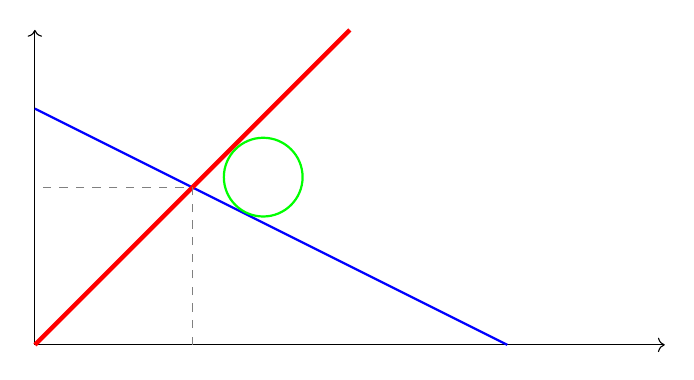
\begin{tikzpicture}[scale=2]
		  \draw [<->] (0,2) -- (0,0) -- (4,0);
		  \draw [blue, thick] (0,1.5) -- (3,0);
		  \draw [red, ultra thick] (0,0) -- (2,2);
		  \draw [dashed, help lines] (1,0) -- (1,1) -- (0,1);
		  \draw [green, thick] (1.45,1.065) circle [radius=0.25];
		\end{tikzpicture}
	\end{center}
\caption{Exemplo simples de gráfico elaborado usando Ti\textit{k}Z.}
\label{fig:tikz-ex1}
\end{figure}

\begin{listing}[ht]
	\begin{minted}[ linenos=true, autogobble, bgcolor=Cornsilk1 ]{tex}
		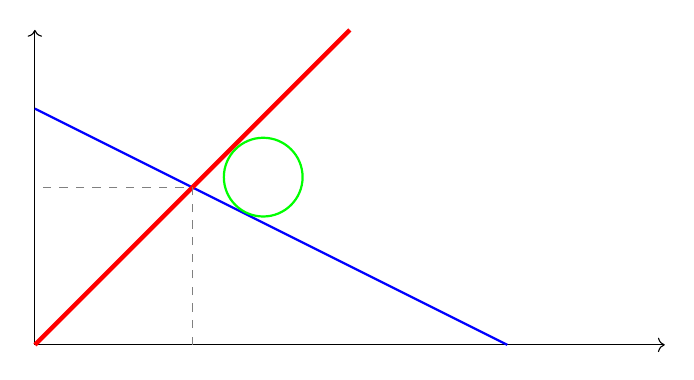
\begin{tikzpicture}[scale=2]
		  \draw [<->] (0,2) -- (0,0) -- (4,0);
		  \draw [blue, thick] (0,1.5) -- (3,0);
		  \draw [red, ultra thick] (0,0) -- (2,2);
		  \draw [dashed, help lines] (1,0) -- (1,1) -- (0,1);
		  \draw [green, thick] (1.45,1.065) circle [radius=0.25];
		\end{tikzpicture}
	\end{minted}
	\caption{Código \LaTeX{} usado para gerar exemplo de gráfico da Figura \ref{fig:tikz-ex1}.}
	\label{cod:cod-tikz-ex1}
\end{listing}

O Ti\textit{k}Z\index{Ti\textit{k}Z} também nos permite desenhar facilmente gráficos de equações como pode ser visto na Figura \ref{fig:tikz-ex2}, que foi gerada com o Código \ref{cod:cod-tikz-ex2}. Observe como é simples se gerar gráficos com funções conhecidas. Caso você queira desenhar gráficos de funções geradas por sequências de pontos, é só carregar as coordenadas dos pontos no formato Ti\textit{k}Z e ligá-los por retas. Note, entretanto, que nesse caso, uma ampliação do pdf iria salientar a falta de suavidade do gráfico, dependendo da amostragem utilizada na geração dos pontos.

\begin{figure}
	\begin{center}
		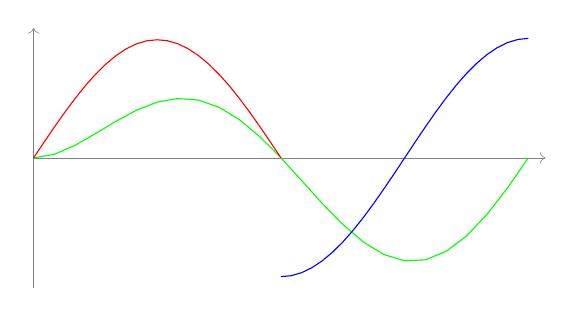
\begin{tikzpicture}[yscale=1.5]
			\draw [help lines, ->] (0,0) -- (6.5,0);
			\draw [help lines, ->] (0,-1.1) -- (0,1.1);
			\draw [green,domain=0:2*pi] plot (\x, {(sin(\x r)* ln(\x+1))/2});
			\draw [red,domain=0:pi] plot (\x, {sin(\x r)});
			\draw [blue, domain=pi:2*pi] plot (\x, {cos(\x r)*exp(\x/exp(2*pi))});
		\end{tikzpicture}
	\end{center}
	\caption{Exemplo de gráfico gerado com Ti\textit{k}Z.}
	\label{fig:tikz-ex2}
\end{figure}

\begin{listing}[ht]
	\begin{minted}[ linenos=true, autogobble, bgcolor=Cornsilk1 ]{tex}
	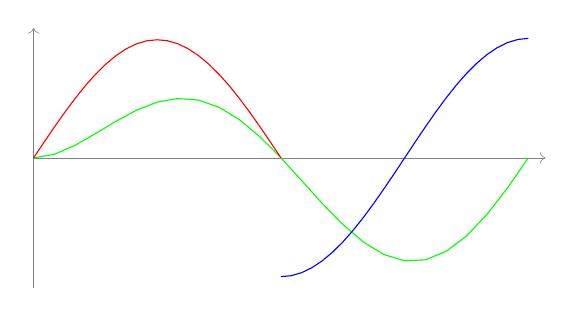
\begin{tikzpicture}[yscale=1.5]
	  \draw [help lines, ->] (0,0) -- (6.5,0);
	  \draw [help lines, ->] (0,-1.1) -- (0,1.1);
	  \draw [green,domain=0:2*pi] plot(\x,{(sin(\x r)*ln(\x+1))/2});
	  \draw [red,domain=0:pi] plot(\x,{sin(\x r)});
	  \draw [blue,domain=pi:2*pi] plot(\x,{cos(\x r)*exp(\x/exp(2*pi))});
	\end{tikzpicture}
	\end{minted}
	\caption{Código \LaTeX{} usado para gerar exemplo de gráfico da Figura \ref{fig:tikz-ex2}.}
	\label{cod:cod-tikz-ex2}
\end{listing}

Os manuais do Ti\textit{k}Z\index{Ti\textit{k}Z} podem ser acessados em \url{http://cremeronline.com/LaTeX/minimaltikz.pdf} \parencite{tikzintro} (manual introdutório) e \url{http://mirrors.ctan.org/graphics/pgf/base/doc/pgfmanual.pdf} \parencite{tikz} (manual oficial). Eu recomendo que tenha o manual oficial do Ti\textit{k}Z, caso precise gerar desenhos com frequência para os seus documentos. Ele é extremamente detalhado e contém muitos exemplos. Além disso, sugiro a página \url{https://texample.net/tikz/examples/}, que armazena muitos exemplos de desenhos gerados com vários pacotes, e que podem servir de base para algum desenho que precise gerar.

\begin{itemize}
	\item SA-Ti\textit{k}Z - O pacote \texttt{sa-tikz}\index{sa-tikz} define a biblioteca Sa-Ti\textit{k}Z que auxilia no desenho de arquiteturas de \textit{switching}\index{switching} (comutação) e define os modelos Clos, Benes e Banyan e algumas variações destes modelos. O pacote permite que se configure aspectos da rede como as dimensões do módulo, a distância entre módulos e a fonte usada. Por exemplo, a Figura \ref{fig:redeBanyan} mostra uma rede de \textit{switching} Banyan-Omega. Para maiores detalhes, consulte o manual, que está disponível em \url{http://mirrors.ctan.org/graphics/pgf/contrib/sa-tikz/doc/sa-tikz-doc.pdf} \parencite{sa-tikz}.

\begin{figure}[htb]
	\begin{center}
        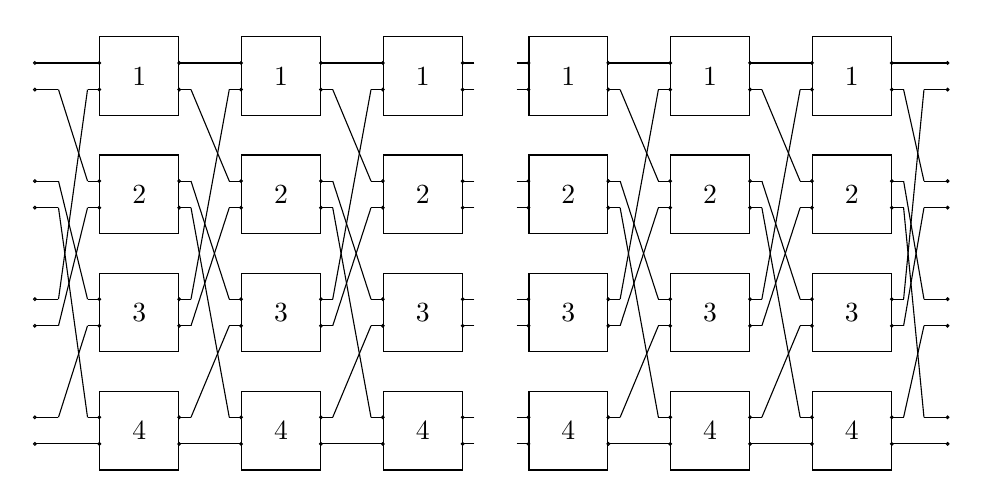
\begin{tikzpicture}
    		% Omega Network on the left
    		\node[banyan omega] {};
    		\begin{scope}[xshift=7.25cm]
	    	% Flip network on the right
	    		\node[banyan flip]{};
    		\end{scope}
		\end{tikzpicture}
	\end{center}
	\caption{Exemplo de duas redes de \textit{switching} Banyan-Omega geradas usando a biblioteca \texttt{switching-architectures} do pacote \texttt{sa-tikz}. Exemplo extraído de \parencite{sa-tikz}.}
	\label{fig:redeBanyan}
\end{figure}

\item Bclogo - O pacote \texttt{bclogo}\index{bclogo} permite que se criem caixas coloridas com a inclusão de logotipos, o que é interessante para chamar a atenção para alguns trechos do documento. Esse pacote depende do pacote \texttt{mdframed}\index{mdframed}. Assim, mensagens importantes, como a mostrada abaixo, podem ter a devida atenção dos leitores.

\begin{bclogo}[
	couleur=bgblue,
	arrondi=0,
	logo=\faBeer,%\bcbombe,
	barre=none,
	noborder=true]{Você Sabia?}
	Você sabia que o consumo moderado de cerveja aumenta a densidade dos ossos em humanos? Um outro estudo mostrou que bebedores moderados têm um menor risco de doenças cardiovasculares do que os abstêmios!
\end{bclogo}

O manual do pacote \texttt{bclogo} (em Francês) pode ser acessado em 
 \url{http://mirrors.ctan.org/graphics/bclogo/doc/bclogo-doc.pdf} \parencite{bclogo}.

\item Ti\textit{k}Z-Dependency\index{Ti\textit{k}Z-Dependency} - O pacote \texttt{tikz-dependency} é um pacote que facilita a criação de grafos de dependência, comumente utilizados em algumas áreas de pesquisa, como grafos e processamento de linguagem natural. 

Ele permite que facilmente se definam estilos para os nós, arestas e rótulos, facilitando enormemente a produção desses grafos. A Figura \ref{fig:grafdep} mostra um exemplo simples feito usando \texttt{tikz-dependency}. Seu manual pode ser acessado em \url{http://mirrors.ctan.org/graphics/pgf/contrib/tikz-dependency/tikz-dependency-doc.pdf} \parencite{tikz-dependency}.

\begin{figure}[htb]
	\begin{center}
	\begin{dependency}[theme=copper]
		\begin{deptext}[column sep=0.2cm]
			My \&[.5cm] dog \& also \&[.7cm] likes \&[.4cm] eating \& sausage \\
		\end{deptext}
		\depedge{2}{1}{poss}
		\depedge{4}{2}{nsubj}
		\depedge{4}{3}{advmod}
		\depedge{4}{5}{xcomp}
		\depedge{5}{6}{dobj}
		\deproot{4}{root}
	\end{dependency}
	\end{center}
	\caption{Exemplo de grafo de dependência criado usando \texttt{tikz-dependency}. Exemplo extraído de \parencite{tikz-dependency}.}
	\label{fig:grafdep}
\end{figure}

\begin{listing}[ht]
	\begin{minted}[ linenos=true, autogobble, bgcolor=Cornsilk1 ]{tex}
	\begin{dependency}[theme=copper]
	  \begin{deptext}[column sep=0.2cm]
	    My \&[.5cm] dog \& also \&[.7cm] likes \&[.4cm] eating 
	    \& sausage \\
	  \end{deptext}
	  \depedge{2}{1}{poss}
	  \depedge{4}{2}{nsubj}
	  \depedge{4}{3}{advmod}
	  \depedge{4}{5}{xcomp}
	  \depedge{5}{6}{dobj}
	  \deproot{4}{root}
	\end{dependency}
	\end{minted}
	\caption{Código \LaTeX{} usado para gerar exemplo de gráfico da Figura \ref{fig:grafdep} usando a biblioteca definida pelo pacote \texttt{tikz-dependency}.}
	\label{cod:cod-grafdep}
\end{listing}

\item Ti\textit{k}Z-Network\index{Ti\textit{k}Z-Network} - Existem várias ferramentas que facilitam o desenho de redes ou grafos, como Xfig\index{Xfig} ou Inkscape\index{Inkscape}. Você pode utilizar uma dessas ferramentas e salvar o conteúdo desejado, de preferência em um formato vetorial, para posteriormente adicioná-las ao seu documento. 

Uma abordagem diferente permite que você desenhe sua rede ou grafo diretamente no documento \LaTeX{}, o que possibilita a realização de ajustes de estilos e tamanhos de fontes, adição de equações, e outras tarefas, sem que se precise retornar a um software externo. O pacote \texttt{tikz-network} permite que se crie e manipule desenhos de redes ou gráficos de maneira simples, gerando gráficos escaláveis que mantêm a qualidade quando o arquivo \gls{pdf}\index{PDF} é ampliado.

A Figura \ref{fig:grafnet} mostra um exemplo simples de rede que foi gerada carregando-se dois arquivos de configuração, um contendo os nós e o outro, as arestas.

\begin{figure}[htb]
	\begin{center}
	\begin{tikzpicture}[scale=1.5]
		\Vertices{./capitulos/vertices.csv}
		\Edges[lw=2.5]{./capitulos/edges.csv}
	\end{tikzpicture}
	\end{center}
	\caption{Exemplo de grafo criado usando \texttt{tikz-network}. Exemplo extraído de \parencite{tikz-network}.}
	\label{fig:grafnet}
\end{figure}

Esse pacote permite que se crie redes mais complexas, como a rede em multinível mostrada na Figura \ref{fig:grafnmn}, que foi gerada usando os comandos vistos no Código \ref{cod:cod-tikz-nmn}. O manual desse pacote pode ser acessado em 
\url{http://mirrors.ctan.org/graphics/pgf/contrib/tikz-network/tikz-network.pdf} \parencite{tikz-network}.

\begin{figure}[htb]
	\begin{center}
	\begin{tikzpicture}[multilayer=3d, scale=1.5]
	  \begin{Layer}[layer=1]
	    \Plane[x=-.5,y=-.5,width=2.5,height=3,grid=5mm]
	  \end{Layer}	 
	  \begin{Layer}[layer=2]
	    \Plane[x=-.5,y=-.5,width=2.5,height=3,grid=5mm]
	    \end{Layer}	
	  \Vertices{capitulos/ml-vertices.csv}
	  \Edges{capitulos/ml-edges.csv}
	\end{tikzpicture}
	\end{center}
\caption{Exemplo de grafo em multinível criado usando \texttt{tikz-network}\index{tikz-network}. Exemplo adaptado de \parencite{tikz-network}\index{tikz-network}.}
\label{fig:grafnmn}
\end{figure}

\begin{listing}[ht]
	\begin{minted}[ linenos=true, autogobble, bgcolor=Cornsilk1 ]{tex}
	\begin{tikzpicture}[multilayer=3d, scale=1.5]
	  \begin{Layer}[layer=1]
	    \Plane[x=-.5,y=-.5,width=2.5,height=3,grid=5mm]
	  \end{Layer}	 
	  \begin{Layer}[layer=2]
	    \Plane[x=-.5,y=-.5,width=2.5,height=3,grid=5mm]
	  \end{Layer}	
	  \Vertices{capitulos/ml-vertices.csv}
	  \Edges{capitulos/ml-edges.csv}
	\end{tikzpicture}
	\end{minted}
	\caption{Código \LaTeX{} usado para gerar exemplo de gráfico da Figura \ref{fig:grafnmn} usando a biblioteca definida pelo pacote \texttt{tikz-network}\index{tikz-network}.}
	\label{cod:cod-tikz-nmn}
\end{listing}

\item PGFPlots - O pacote \texttt{pgfplots}\index{PGFPlots} permite criar facilmente gráficos de alta qualidade em escalas lineares e logarítmicas em 2D e 3D usando uma interface amigável. A Figura \ref{fig:pgfplots} mostra um gráfico gerado usando esse pacote, com a sequência de comandos mostradas no código \ref{cod:pgfplots}.

% Preamble: \pgfplotsset{width=7cm,compat=1.17}
\begin{figure}[H]
	\begin{center}
		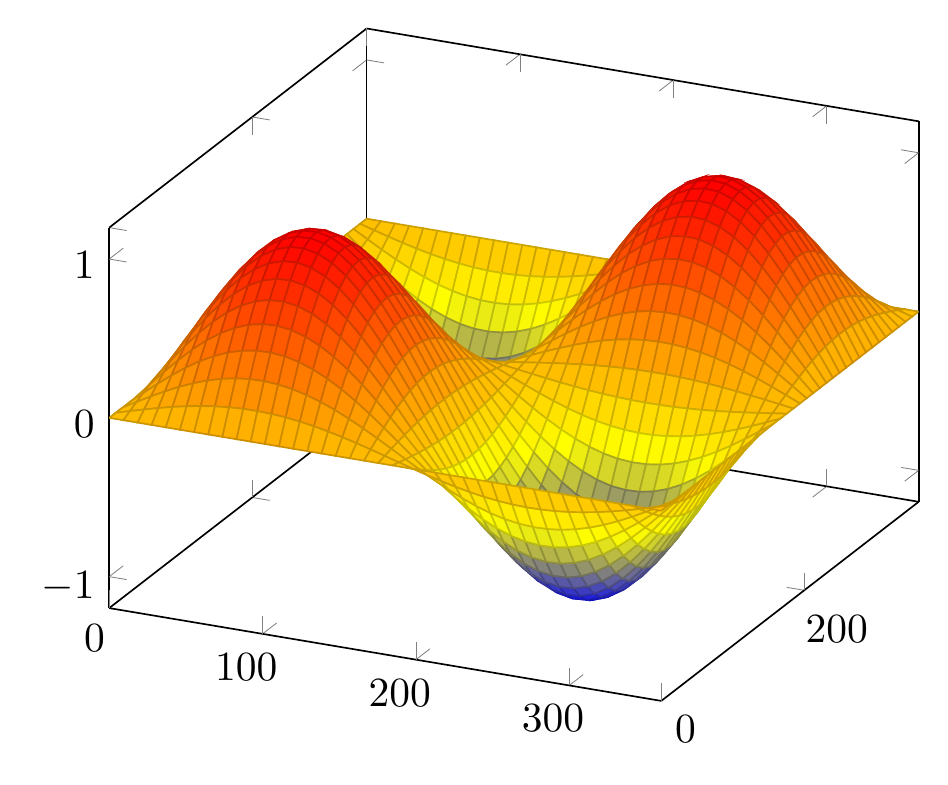
\begin{tikzpicture}[scale=1.5]
			\begin{axis}
				\addplot3 [ surf, domain=0:360,	samples=40,	] {sin(x)*sin(y)};
			\end{axis}
		\end{tikzpicture}
	\end{center}
	\caption{Exemplo de gráfico 3D impresso usando \texttt{pgfplots}\index{PGFPlots}.}
	\label{fig:pgfplots}
\end{figure}

\begin{listing}[ht]
	\begin{minted}[ linenos=true, autogobble, bgcolor=Cornsilk1 ]{tex}
		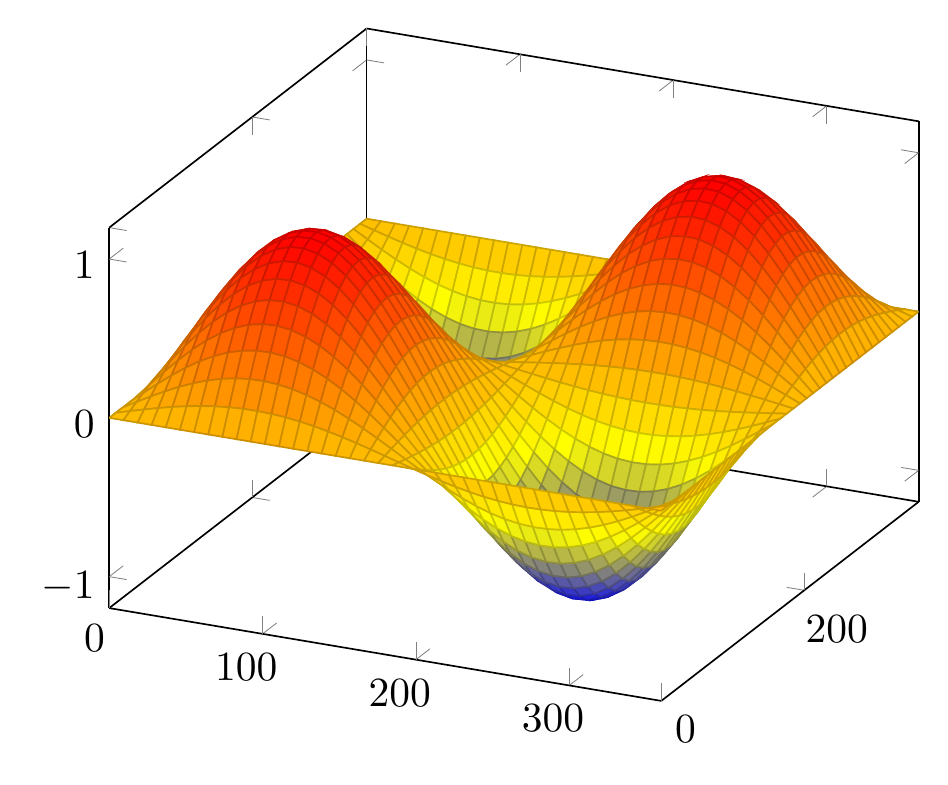
\begin{tikzpicture}[scale=1.5]
		  \begin{axis}
		    \addplot3 [ surf, domain=0:360, samples=40, ] {sin(x)*sin(y)};
		  \end{axis}
		\end{tikzpicture}
	\end{minted}
	\caption{Código \LaTeX{} usado para gerar exemplo de gráfico da Figura \ref{fig:pgfplots} usando o pacote \texttt{pgfplots}\index{PGFPlots}.}
	\label{cod:pgfplots}
\end{listing}

Algumas rotinas chamadas por este pacote, principalmente as 3D, podem ser demoradas, acarretando em aumento razoável do tempo de compilação do seu documento. Deste modo, analise se esta é a melhor opção ou se você deveria gerar os gráficos 3D fora do \LaTeX{} e importá-los.

O manual desse pacote pode acessado em \url{http://mirrors.ctan.org/graphics/pgf/contrib/pgfplots/doc/pgfplots.pdf} \parencite{pgfplots}, e muitos exemplos podem ser encontrados na Internet.

\item Como mais um exemplo de tipo específico de desenho, apresento uma figura gerada com o auxílio da bilbioteca \texttt{mindmaps}\index{mindmaps}. Essa biblioteca pode ser usada juntamente com o Ti\textit{k}Z para criar mapas mentais, que são diagramas usados para organizar informações visualmente. A Figura \ref{fig:mapamental} mostra um exemplo que elenca os capítulos desse documento, detalhando as subseções de alguns capítulos.

Certos cuidados devem ser tomados ao criar esses mapas mentais. Muitos ramos ou textos longos criam problemas na diagramação, que devem ser corrigidos alterando a escala e os ângulos entre os ramos. Mais detalhes podem ser acessados no tutorial para iniciantes em Ti\textit{k}Z do \gls{overleaf}\index{Overleaf}, que pode ser acessado em \url{https://www.overleaf.com/learn/latex/LaTeX_Graphics_using_TikZ:_A_Tutorial_for_Beginners_(Part_5)\%E2\%80\%94Creating_Mind_Maps}.

\begin{figure}[htb]
	\begin{center}
	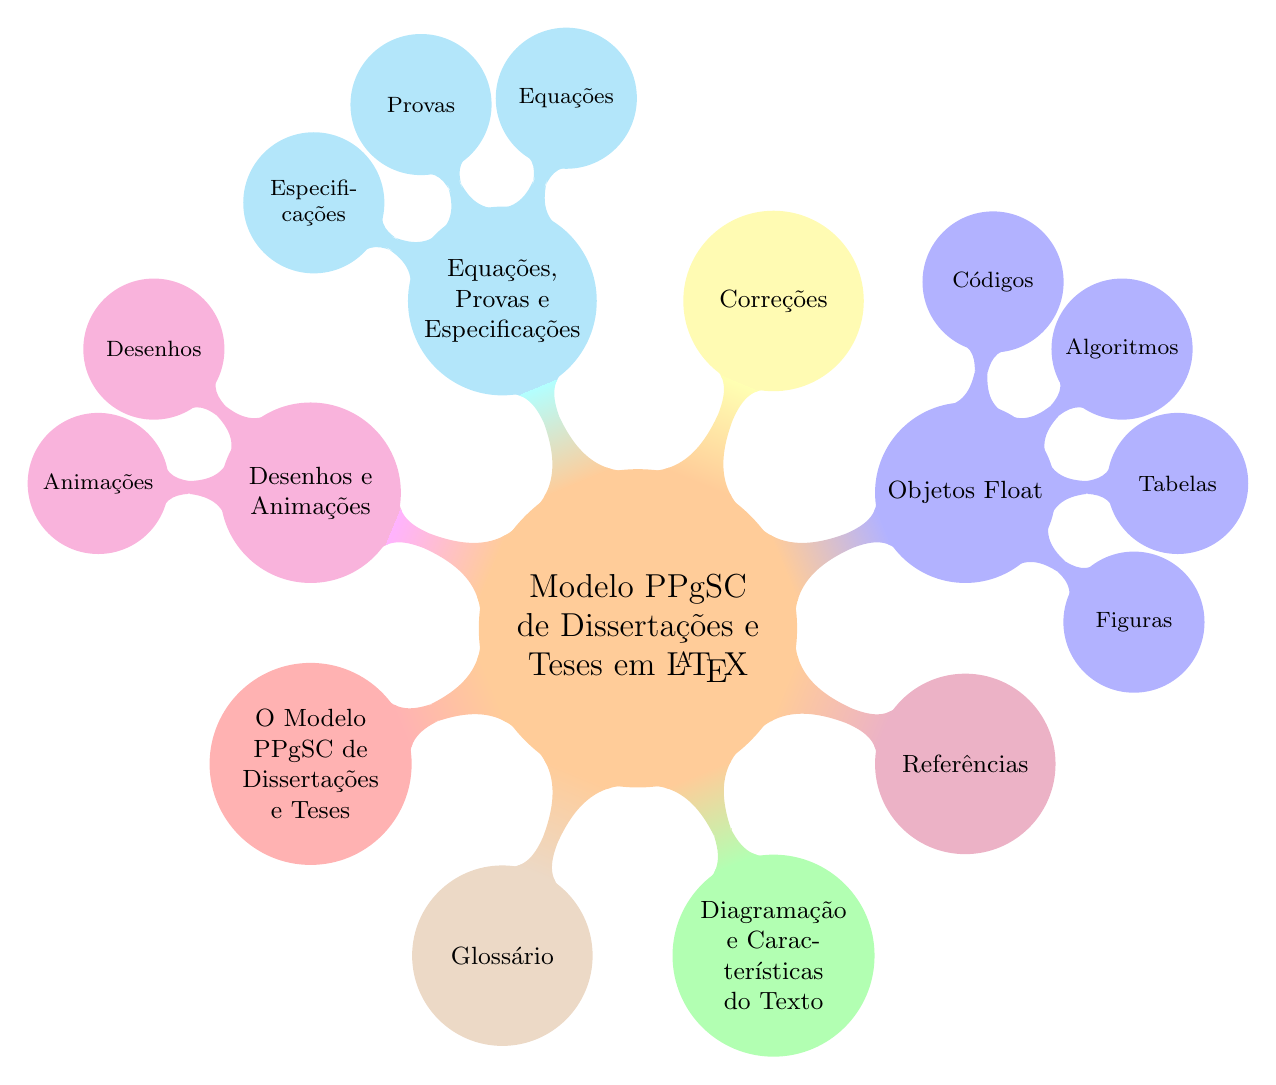
\begin{tikzpicture}[mindmap, scale=0.9, grow cyclic, every node/.style=concept, concept color=orange!40, 
	level 1/.append style={level distance=5cm,sibling angle=45},
	level 2/.append style={level distance=3cm,sibling angle=40}]

    \node{Modelo PPgSC de Dissertações e Teses em \LaTeX{}}
    child [concept color = red!30] { node {O Modelo PPgSC de Dissertações e Teses}
%            child {node {Pacotes}}
%            child {node {Codificação de Entrada e Fontes}}
%            child {node {Estrutura de Arquivos}}
%            child {node {Linguagens}}
%            child {node {Variáveis}}
    }
	child [concept color = brown!30] { node {Glossário}
	}
	child [concept color = green!30] { node {Diagramação e Características do Texto}
%			child {node {Espaça\-mento e Indentação}}
%			child {node {Ajustes Finos}}
%			child {node {Cores}}
%			child {node {Contadores}}
%			child {node {Listas}}
	}
	child [concept color = purple!30] { node {Referências}
	}
	child [concept color = blue!30] { node {Objetos Float}
			child {node {Figuras}}
			child {node {Tabelas}}
			child {node {Algoritmos}}
			child {node {Códigos}}
	}
	child [concept color = yellow!30] { node {Correções}
	}
	child [concept color = cyan!30] { node {Equações, Provas e Especificações}
			child {node {Equações}}
			child {node {Provas}}
			child {node {Especifi\-cações}}
	}
	child [concept color = magenta!30] { node {Desenhos e Animações}
			child {node {Desenhos}}
			child {node {Animações}}
	}
;
	\end{tikzpicture}
\end{center}
\caption{Exemplo de mapa mental criado usando biblioteca \texttt{mindmaps} para Ti\textit{k}Z. O mapa mostra todos os capítulos contidos neste documento e expande alguns capítulos em suas seções.}
\label{fig:mapamental}
\end{figure}

\item Ti\textit{k}Z-3dplots - O pacote \texttt{tikz-3dplot}\index{tikz-3dplot} permite definir sistemas de coordenadas tridimensionais para uso com desenhos Ti\textit{k}Z\index{Ti\textit{k}Z}. O usuário pode especificar a orientação do sistema de coordenadas principal para desenhar e um segundo sistema de coordenadas para realizar rotações e translações em relação ao sistema de coordenadas principal. O pacote ainda permite que se use coordenadas polares esféricas para desenhar.

É importante ressaltar que tudo o que você pode fazer com o pacote \texttt{tikz-3dplot}\index{tikz-3dplot} pode ser feito usando Ti\textit{k}Z puro. A ideia é a de que o pacote \texttt{tikz-3dplot} facilita a tarefa de criação de desenhos tridimensionais e suas projeções bidimensionais. 

Antes de desenhar uma figura, você deve definir a transformação para o sistema de coordenadas principal, que determina a posição da câmera virtual, além de definir varáveis que serão utilizadas em seus desenhos. Os comandos mostrados no Código \ref{cod:3dplot-setup} mostram as definições da posição da câmera virtual e de três ângulos.

\begin{listing}[ht]
	\begin{minted}[ linenos=true, autogobble, bgcolor=Cornsilk1 ]{tex}
		\begin{tikzpicture}[scale=5,tdplot_main_coords]
			\tdplotsetmaincoords{60}{110}
			\pgfmathsetmacro{\rvec}{.8}
			\pgfmathsetmacro{\thetavec}{30}
			\pgfmathsetmacro{\phivec}{60}
		\end{tikzpicture}
	\end{minted}
	\caption{Código Ti\textit{k}Z, contendo comandos definidos no pacote \texttt{tikz-3dplot}, usado para gerar a Figura \ref{fig:3dplot}}
	\label{cod:3dplot-setup}
\end{listing}

A Figura \ref{fig:3dplot} mostra um exemplo de gráfico produzido usando esse pacote, enquanto que o Código \ref{cod:3dplot} apresenta o código usado para desenhá-lo.  

\tdplotsetmaincoords{60}{110}
%
\pgfmathsetmacro{\rvec}{.8}
\pgfmathsetmacro{\thetavec}{30}
\pgfmathsetmacro{\phivec}{60}
%
\begin{figure}[ht]
	\begin{center}
\begin{tikzpicture}[scale=5,tdplot_main_coords]
  \coordinate (O) at (0,0,0);
  \draw[thick,->] (0,0,0) -- (1,0,0) node[anchor=north east]{$x$};
  \draw[thick,->] (0,0,0) -- (0,1,0) node[anchor=north west]{$y$};
  \draw[thick,->] (0,0,0) -- (0,0,1) node[anchor=south]{$z$};
  \tdplotsetcoord{P}{\rvec}{\thetavec}{\phivec}
  \draw[-stealth,color=red] (O) -- (P);
  \draw[dashed, color=red] (O) -- (Pxy);
  \draw[dashed, color=red] (P) -- (Pxy);
  \tdplotdrawarc{(O)}{0.2}{0}{\phivec}{anchor=north}{$\phi$}
  \tdplotsetthetaplanecoords{\phivec}
  \tdplotdrawarc[tdplot_rotated_coords]{(0,0,0)}{0.5}{0}%
    {\thetavec}{anchor=south west}{$\theta$}
  \draw[dashed,tdplot_rotated_coords] (\rvec,0,0) arc (0:90:\rvec);
  \draw[dashed] (\rvec,0,0) arc (0:90:\rvec);
  \tdplotsetrotatedcoords{\phivec}{\thetavec}{0}
  \tdplotsetrotatedcoordsorigin{(P)}
  \draw[thick,tdplot_rotated_coords,->] (0,0,0)
 	-- (.5,0,0) node[anchor=north west]{$x’$};
  \draw[thick,tdplot_rotated_coords,->] (0,0,0)
 	-- (0,.5,0) node[anchor=west]{$y’$};
  \draw[thick,tdplot_rotated_coords,->] (0,0,0)
 	-- (0,0,.5) node[anchor=south]{$z’$};
  \draw[-stealth,color=blue,tdplot_rotated_coords] (0,0,0) -- (.2,.2,.2);
  \draw[dashed,color=blue,tdplot_rotated_coords] (0,0,0) -- (.2,.2,0);
  \draw[dashed,color=blue,tdplot_rotated_coords] (.2,.2,0) -- (.2,.2,.2);
  \tdplotdrawarc[tdplot_rotated_coords,color=blue]{(0,0,0)}{0.2}{0}%
  {45}{anchor=north west,color=black}{$\phi’$}
  \tdplotsetrotatedthetaplanecoords{45}
  \tdplotdrawarc[tdplot_rotated_coords,color=blue]{(0,0,0)}{0.2}{0}%
  {55}{anchor=south west,color=black}{$\theta’$}
 \end{tikzpicture}
 \end{center}
\caption{Exemplo de desenho produzido com o auxílio do pacote \texttt{tikz-3dplot}.  Exemplo extraído de \parencite{tikz-3dplot}.}
\label{fig:3dplot}
\end{figure}

O manual do \texttt{tikz-3dplot}\index{tikz-3dplot} pode ser acessado em
\url{http://mirrors.ctan.org/graphics/pgf/contrib/tikz-3dplot/tikz-3dplot_documentation.pdf} \parencite{tikz-3dplot}. Existem vários \textit{threads} de questões sobre desenhos 3D usando Ti\textit{k}Z na área de \TeX{} do StackExchange\index{StackExchange} \url{https://stackexchange.com}, seja com o auxílio de \texttt{tikz-3dplot} ou não. Recomendo que faça uma busca não só nessa página, mas também em páginas como a do \TeX{}ample.net (\url{https://texample.net/}) antes de começar a criar seus gráficos 3D.

\begin{listing}[H]
	\begin{minted}[ linenos=true, autogobble, bgcolor=Cornsilk1 ]{tex}
		\begin{tikzpicture}[scale=5,tdplot_main_coords]
		  \coordinate (O) at (0,0,0);
		  \draw[thick,->] (0,0,0) -- (1,0,0) node[anchor=north east]{$x$};
		  \draw[thick,->] (0,0,0) -- (0,1,0) node[anchor=north west]{$y$};
		  \draw[thick,->] (0,0,0) -- (0,0,1) node[anchor=south]{$z$};
		  \tdplotsetcoord{P}{\rvec}{\thetavec}{\phivec}
		  \draw[-stealth,color=red] (O) -- (P);
		  \draw[dashed, color=red] (O) -- (Pxy);
		  \draw[dashed, color=red] (P) -- (Pxy);
		  \tdplotdrawarc{(O)}{0.2}{0}{\phivec}{anchor=north}{$\phi$}
		  \tdplotsetthetaplanecoords{\phivec}
		  \tdplotdrawarc[tdplot_rotated_coords]{(0,0,0)}{0.5}{0}%
		  {\thetavec}{anchor=south west}{$\theta$}
		  \draw[dashed,tdplot_rotated_coords] (\rvec,0,0) arc (0:90:\rvec);
		  \draw[dashed] (\rvec,0,0) arc (0:90:\rvec);
		  \tdplotsetrotatedcoords{\phivec}{\thetavec}{0}
		  \tdplotsetrotatedcoordsorigin{(P)}
		  \draw[thick,tdplot_rotated_coords,->] (0,0,0)
		  -- (.5,0,0) node[anchor=north west]{$x’$};
		  \draw[thick,tdplot_rotated_coords,->] (0,0,0)
		  -- (0,.5,0) node[anchor=west]{$y’$};
		  \draw[thick,tdplot_rotated_coords,->] (0,0,0)
		  -- (0,0,.5) node[anchor=south]{$z’$};
		  \draw[-stealth,color=blue,tdplot_rotated_coords] (0,0,0) --(.2,.2,.2);
		  \draw[dashed,color=blue,tdplot_rotated_coords] (0,0,0) -- (.2,.2,0);
		  \draw[dashed,color=blue,tdplot_rotated_coords] (.2,.2,0) --(.2,.2,.2);
		  \tdplotdrawarc[tdplot_rotated_coords,color=blue]{(0,0,0)}{0.2}{0}%
		  {45}{anchor=north west,color=black}{$\phi’$}
		  \tdplotsetrotatedthetaplanecoords{45}
		  \tdplotdrawarc[tdplot_rotated_coords,color=blue]{(0,0,0)}{0.2}{0}%
		  {55}{anchor=south west,color=black}{$\theta’$}
		\end{tikzpicture}
	\end{minted}
	\caption{Código Ti\textit{k}Z, contendo comandos definidos no pacote \texttt{tikz-3dplot}, usado para gerar a Figura \ref{fig:3dplot}}
	\label{cod:3dplot}
\end{listing}

%\item Forest - O pacote \texttt{forest}

\item Ti\textit{k}Z-qtree - O pacote \texttt{tikz-qtree}\index{tikz-qtree} implementa uma parte dos comandos do pacote \texttt{qtree} usando Ti\textit{k}Z\index{Ti\textit{k}Z}. A sintaxe é a mesma do \texttt{qtree}, e segundo os autores, as características mais básicas daquele pacote estão implementadas. Além disso, comandos Ti\textit{k}Z podem ser incorporados na descrição das árvores. O manual desse pacote pode ser acessado em \url{http://mirrors.ctan.org/graphics/pgf/contrib/tikz-qtree/tikz-qtree-manual.pdf} \parencite{tikz-qtree}.

\item Animate - O pacote \texttt{animate} permite criar animações em \gls{pdf}\index{PDF} usando JavaScript\index{JavaScript} e em \gls{svg}\index{SVG}. Infelizmente, este pacote só funciona os visualizadores \gls{pdf} que suportam JavaScript\index{JavaScript}, como o Acrobat Reader \faCopyright. No caso de animações \gls{svg}, essa ferramenta permite que elas sejam usadas em navegadores. Essa pode ser uma poderosa ferramenta na demostração de algo dinâmico. Para os interessados, sugiro que estudem e testem os exemplos do manual desse pacote, acessível em \url{http://mirrors.ctan.org/macros/latex/contrib/animate/animate.pdf} \parencite{animate}.

\item  Outros pacotes - Existem vários outros pacotes de desenho que se baseiam no Ti\textit{k}Z disponíveis gratuitamente, mas que não estão armazenados no \gls{ctan}. Um deles é o  \texttt{tkz-2d}\index{tkz-2d}, que pode ser baixado de \url{https://texample.net/tikz/examples/tkz-2d/} \parencite{tkz-2d}. Além disso, temos várias bibliotecas prontas para uso com o Ti\textit{k}Z, como a \texttt{decoration.fractals}, que nos permite desenhar facilmente curvas fractais como a curva de Koch de níveis 0, 1, 2 e 3, mostradas na Figura \ref{fig:kochcurve}.

\begin{figure}[H]
	\begin{center}
	\begin{tabular}{|c|c|c|c|} \hline 
		\begin{tikzpicture}[decoration=Koch snowflake,draw=blue,fill=blue!20,thick]
		  \filldraw  (0,0) -- ++(60:3) -- ++(-60:3) -- cycle ;
		\end{tikzpicture}
		& 
	
		\begin{tikzpicture}[decoration=Koch snowflake,draw=blue,fill=blue!20,thick]
		  \filldraw decorate{ (0,0) -- ++(60:3) -- ++(-60:3) -- cycle };
		
		\end{tikzpicture}
		&  
		\begin{tikzpicture}[decoration=Koch snowflake,draw=blue,fill=blue!20,thick]
		  \filldraw decorate{ decorate{ (0,0) -- ++(60:3) -- ++(-60:3) -- cycle }};
		\end{tikzpicture}
		&  
		\begin{tikzpicture}[decoration=Koch snowflake,draw=blue,fill=blue!20,thick]
		  \filldraw decorate{ decorate{ decorate{ (0,0) -- ++(60:3) -- ++(-60:3) -- cycle }}};
		\end{tikzpicture}
		\\ \hline  
		Nível 0 & Nível 1 &  Nível 2 &  Nível 3 \\ \hline
	\end{tabular}
	\end{center}
	\caption{Exemplo de grafo em multinível criado usando \texttt{tikz-network}. Exemplo extraído de \url{http://mirrors.ctan.org/info/visualtikz/VisualTikZ.pdf}.}
	\label{fig:kochcurve}
\end{figure}
		
Os comandos necessários para desenhar as curvas e organizá-las no ambiente tabular podem ser vistos no Código \ref{cod:cod-kochcurve}. Note a simplicidade e elegância do código recursivo usado para desenhar as curvas.

\begin{listing}[ht]
	\begin{minted}[linenos=true, autogobble, bgcolor=Cornsilk1]{tex}
		\begin{center}
		\begin{tabular}{|c|c|c|c|} \hline 
		  \begin{tikzpicture}[decoration=Koch snowflake,draw=blue,
		  	            fill=blue!20,thick]
		    \filldraw  (0,0) -- ++(60:3) -- ++(-60:3) -- cycle ;
		  \end{tikzpicture}
		  & 
		  \begin{tikzpicture}[decoration=Koch snowflake,draw=blue,
		  	            fill=blue!20,thick]
		    \filldraw decorate{ (0,0) -- ++(60:3) -- ++(-60:3) -- cycle };
		  \end{tikzpicture}
		  &  
		  \begin{tikzpicture}[decoration=Koch snowflake,draw=blue,
		  	            fill=blue!20,thick]
		    \filldraw decorate{ decorate{ (0,0) -- ++(60:3) -- ++(-60:3) 
		              -- cycle }};
		  \end{tikzpicture}
		  &  
		  \begin{tikzpicture}[decoration=Koch snowflake,draw=blue,
		  	            fill=blue!20,thick]
		    \filldraw decorate{ decorate{ decorate{ (0,0) -- ++(60:3) 
		              -- ++(-60:3) -- cycle }}};
		  \end{tikzpicture}
		  \\ \hline  
		  Nível 0 & Nível 1 &  Nível 2 &  Nível 3 \\ \hline
		\end{tabular}
		\end{center}
	\end{minted}
	\caption{Código \LaTeX{} usado para gerar exemplos de curvas fractais da Figura \ref{fig:kochcurve} usando a biblioteca decoration.fractal do Ti\textit{k}Z.}
	\label{cod:cod-kochcurve}
\end{listing}

\end{itemize}

Eu recomendo que sempre que precise desenhar algo mais complexo em Ti\textit{k}Z, faça uma busca na Internet para avaliar se não existe algum código disponível que possa ajudá-lo. Em alguns casos, existem vários pacotes que têm propostas similares, como os pacotes \texttt{forest}\index{forest} e \texttt{tikz-qtree}\index{tikz-qtree}. Nestes caso, você deve pesquisar e definir qual é a melhor opção para você. 

Outra possibilidade é a utilização de ferramentas de desenho que salvam em formato Ti\textit{k}Z\index{Ti\textit{k}Z}. Existem várias ferramentas que permitem se criar desenhos vetoriais e salvá-los na linguagem Ti\textit{k}Z. Dentre estas, destaco a Geogebra (\url{https://www.geogebra.org/}), uma ótima ferramenta para criar e visualizar funções, objetos geométricos e superfícies, e que possui uma página introdutória no \gls{overleaf} ensinando a gerar código Ti\textit{k}Z. Além dela, você pode utilizar as ferramentas TikZit\index{TikZit} (\url{https://tikzit.github.io/}) e TikzEdt\index{TikzEdt} (\url{http://www.tikzedt.org/}), que permitem que você crie ilustrações usando linguagem Ti\textit{k}Z ou comandos interativos, e visualize os efeitos das alterações imediatamente.

Uma outra possibilidade é a utilização do Inkscape\index{Inkscape}, um programa de desenho vetorial, que salva os desenhos em formato \gls{svg}\index{SVG}, seguido da conversão dos arquivos SVG em Ti\textit{k}Z\index{Ti\textit{k}Z} usando uma ferramenta externa, como o SGV2TikZ\index{SGV2TikZ} \url{https://github.com/xyz2tex/svg2tikz} já que o Inkscape não dá mais suporte a essas conversões.

\section{Asymptote} \label{asymptote}

Asymptote\index{Asymptote} é uma poderosa linguagem descritiva de gráficos vetoriais para desenhos técnicos. Ela foi inspirada em \hologo{METAPOST}\index{\hologo{METAPOST}} mas possui uma sintaxe parecida com C++. Os programas escritos em Asymptote devem ser processados usando o programa \texttt{asy}\index{asy}, que gerará uma saída no formato \gls{eps}\index{EPS} (default) ou no formato \gls{pdf}\index{PDF} (caso explicitamente especificado). Abaixo vemos as chamadas usadas para processar o arquivo \texttt{test.asy} em uma saída dos tipos \gls{eps} e \gls{pdf}. 

\begin{adjustbox}{fbox, center, tabular=l, vspace=0.5cm}
	\texttt{asy -V test} \\
	\texttt{asy -V -f pdf test}
\end{adjustbox}

Entretanto, o Asymptote, permite que se coloque o código Asymptote dentro do arquivo \LaTeX{}, encapsulado no ambiente \texttt{asy}\index{asy}. Então, após o processamento do arquivo pelo processador \LaTeX{}, o Asymptote deve ser executado e depois o o processador \LaTeX{} deve ser executado novamente, como visto abaixo. Lembro novamente, que este fluxo de processamento deve ser escolhido nas opções de sua ferramenta de edição \LaTeX{} ou executado diretamente na linha de comando. 

\begin{adjustbox}{fbox, center, tabular=l, vspace=0.5cm}
	\texttt{pdflatex DissertacaoPPgSC} \\
	\texttt{asy DissertacaoPPgSC-*.asy} \\
	\texttt{pdflatex DissertacaoPPgSC} 
\end{adjustbox}

Diferente do Ti\textit{k}Z, o Asymptote\index{Asymptote} usa a unidade de tamanho ponto (\texttt{point}), que equivale a 0,035$cm$. Para usar centímetro como a unidade do Asymptote, deve-se usar o comando abaixo:

\adjustbox{fbox, center}{\texttt{unitsize(1cm);}}

A Figura \ref{fig:beziersub} mostra um exemplo de gráfico gerado usando Asymptote, que representa o algoritmo recursivo de subdivisão de curvas de Bézier. Neste caso, optei por gerar o gráfico em formato \gls{pdf}\index{PDF} fora da ferramenta \LaTeX{} e importá-la usando o comando \texttt{\textbackslash includegraphics}.

\begin{figure}[H]
	\centering
	\includegraphics[scale=1]{imagens/capitulo5/bezier2.pdf}
	\caption{Ilustração do algoritmo recursivo de subdivisão de curvas de Bézier.}
	\label{fig:beziersub}
\end{figure}

O Código \ref{cod:asymptote} mostra os comandos em Asymptote usados para gerar a Figura \ref{fig:beziersub}. Note como é simples e intuitivo desenhar retas e posicionar os nomes dos pontos, e a definição da função auxiliar \texttt{midpoint}. 

\begin{listing}[ht]
	\begin{minted}[linenos=true, autogobble, bgcolor=Cornsilk1]{asy}
	import beziercurve;

	pair midpoint(pair a, pair b) {return interp(a,b,0.5);}

	pair m0=midpoint(z0,c0);
	pair m1=midpoint(c0,c1);
	pair m2=midpoint(c1,z1);

	draw(m0--m1--m2,dashed);
	dot("$m_0$",m0,NW,red);
	dot("$m_1$",m1,N,red);
	dot("$m_2$",m2,red);

	pair m3=midpoint(m0,m1);
	pair m4=midpoint(m1,m2);
	pair m5=midpoint(m3,m4);

	draw(m3--m4,dashed);
	dot("$m_3$",m3,NW,red);
	dot("$m_4$",m4,NE,red);
	dot("$m_5$",m5,N,red);
	\end{minted}
	\caption{Código Asymptote usado para gerar a Figura \ref{fig:beziersub}.}
	\label{cod:asymptote}
\end{listing}



O Asymptote também permite que se construa animações dos gráficos gerados usando seu pacote \texttt{animation}\index{animation}, que empilha múltiplas imagens em um \gls{gif}\index{GIF} animado ou um vídeo \gls{mpeg}\index{MPEG} usando o programa \texttt{convert} do software ImageMagick. Assim como no caso do Ti\textit{k}Z, essas animações só podem ser visualizadas em leitores de \gls{pdf}\index{PDF} que suportem JavaScript\index{JavaScript} ou em browsers.

O Asymptote provê uma interface gráfica bem simples, a \texttt{xasy}\index{xasy}, que permite que se veja imediatamente o resultado da manipulação dos elementos gráficos. Como a interface não é tão completa, o usuário pode preferir salvar o código do gráfico e completar a programação fora da ferramenta.

Uma boa referência inicial é o tutorial disponível em \url{https://asymptote.sourceforge.io/asymptote_tutorial.pdf} \parencite{asymptotetut}. Caso precise de informações mais detalhadas, você pode acessar o manual do Asymptote\index{Asymptote} em \url{http://mirrors.ctan.org/graphics/asymptote/doc/asymptote.pdf} \parencite{asymptote}. Finalmente, você também pode obter o cartão de referência dos comandos Asymptote no endereço \url{http://mirrors.ctan.org/graphics/asymptote/doc/asyRefCard.pdf} \parencite{asymptoterefcard}. 


